\chapter{Proofs}

\section{Measures on parallelogram grid dispersion} \label{sec:proof_pargrid_measures}

The parallelogram side lengths $x, y$ can be calculated in function of $p_x$, $p_y$, and the normal vector $\vec{n}$ using
\begin{equation}
x = p_x \, \sqrt{1 + \frac{n^2_x}{n^2_z}}
\hspace{7mm} \text{and} \hspace{7mm}
y = p_y \, \sqrt{1 + \frac{n^2_y}{n^2_z}}
\end{equation}
When $\vec{n} = \transpose{(0, 0, 1)}$, the plane is perpendicular to the camera ray, and it can be seen that $x = p_x, y = p_y$. Also the ratios $\frac{x}{p_x}$ and $\frac{x}{p_x}$ depend only on $\vec{n}$.

\begin{proof}
The parallelogram side lengths $x, y$ can be calculated in function of $p_x$, $p_y$, and the normal vector $\vec{n}$. Let $\vec{x}$ be the projection of $\vec{p_x} = \transpose{(p_x, 0, 0)}$ on the plane. $\vec{x}$ lies on the plane and is orthogonal to $\vec{n}$, so $\vec{n} \, \vec{x} = 0$ and $n_x x_x + n_y x_y + n_z x_z = 0$. $\vec{x}$ also lies on the XZ-plane, so $x_y = 0$. By projection $x_x = p_x$. Solving the dot product equation, $x_z = -\frac{n_x}{n_z} \, p_x$. So
\begin{equation}
\vec{x} = \left( \begin{matrix}
	p_x \\
	0 \\
	-\frac{n_x}{n_z} \, p_x
\end{matrix} \right)
\end{equation}
The side lengths $x$ is
\begin{equation}
x = \| \vec{x} \| = \sqrt{p^2_x + \left( \frac{n_x}{n_z} \, p_x \right)^2} = p_x \, \sqrt{1 + \frac{n^2_x}{n^2_z}}
\end{equation}
And $y$ can be obtained in the same manner.
\end{proof}




\section{Closest point histogram with random point dispersion on plane} \label{sec:proof_rand_disp_plane}
Point clouds $P$ and $Q$ are two perfectly aligned planes, the points $p \in P$ are randomly dispersed on $P$. $Q$ contains a large number of sample points. The probability density function for the distance of a random point $q \in Q$ to its closest neighbor in $P$ is given by
\begin{equation}
f_R(r) = 2 \pi \rho(P) \, r \, e^{-\pi \rho(P) \, r^2}
\end{equation}

\begin{proof}
Let $P$ be a bounded continuous surface in $\mathbb{R}^2$ of area $\area{P}$. For the example on the figure \ref{fig:plane_rand_d30000}, it is a square with side length $5$. Let $\{ p_i \in P \}$ be a discrete set of $n$ randomly chosen points on that surface, with an uniform probability distribution. $\rho = \frac{n}{\area{P}}$ is the surface density of this points distribution.

Let $A \subset W$ a another bounded continuous subregion of $P$, with a variable area $\area{A}$ on the order of magnitude of the distances between adjacent neighboring points $p_i$. Let $N(A) \in \mathbb{N}$ be the number of points $p_i \in P$ that lie inside $A$. In the following formulas, the area value $\area{A}$ is also denoted $A$.

For any single point $p_i \in P$, the probability that it lies in $A$, and the probability that it does not, are given by
\begin{equation} \label{eq:rand_point_in_A}
P[p_i \in A] = \frac{\area{A}}{\area{P}} = \frac{A \rho}{n}
\hspace{7mm} \text{and} \hspace{7mm}
P[p_i \notin A] = 1 - \frac{A \rho}{n}
\end{equation}

For any two $p_i$, these events are stochastically independent, and the probability that two events occur is obtained through multiplication. The probability that none of the $n$ points lie in $A$, and conversely the probability that at least one lies in $A$, are;

\begin{equation}
P[N(A) = 0] = \left(1 - \frac{A \rho}{n}\right)^n
\hspace{7mm} \text{and} \hspace{7mm}
P[N(A) \geq 1] = 1 - \left(1 - \frac{A \rho}{n}\right)^n
\end{equation}


The value $P[N(A) \geq 1]$ converges for $n \rightarrow \infty$. The information about the density of points is captured by $\rho$, so the probability be be expressed without $\area{P}$ and $n$. Setting $n' = -\frac{n}{A \, \rho}$ and using the identity $\lim_{x \rightarrow \infty} \left( 1 + \frac{1}{x} \right)^x = e$:
\begin{equation}
\begin{align}
\lim_{n \rightarrow \infty} P[N(A) \geq 1]
& = \lim_{n \rightarrow \infty} \left[ 1 - \left(1 - \frac{A \rho}{n}\right)^n \right]\\
& = 1 - \lim_{n \rightarrow \infty} \left(1 - \frac{A \rho}{n}\right)^n \\
& = 1 - \lim_{n' \rightarrow \infty} \left(1 + \frac{1}{n'}\right)^{-A \rho \, n'}\\
& = 1 - \left[ \lim_{n' \rightarrow \infty} \left(1 + \frac{1}{n'}\right)^{n'} \right]^{-A \rho}\\
& = 1 - e^{-A \rho}
\end{align}
\label{eq:leastone_point_prob}
\end{equation}
For the final expression $A \in \mathbb{R}$ denotes only the area, as no further information on the region's shape is needed. 

The goal what to find the underlying curve of the histogram in \ref{fig:plane_rand_d30000}. In order to obtain a smooth function, the histogram taken with a sparse set of points $q \in Q$ is replaced by a probability density function of the closest point distance from any $q \in Q$ to its nearest neighbor $p_i \in P$. The surfaces $P$ and $Q$ are the same.

Let $q \in P$ be any point lying on the plane $P$. (Not necessarily one of the discrete set of points $p_i$.) Let $D_{q,r} \in P$ be the disk centered at $q$ with radius $r$. Its area is $\area{D_{r}} = \pi r^2$. By definition, for any point $p \in D_{q,r}$, $\| p - q \| \leq r$. Starting from $r = 0$, the radius of the disk is increased until $N(D_{q,r}) = 1$. $r = r_{\text{closest}}$ is then the closest point distance to $q$.

One has $r \geq r_{\text{closest}}$ if and only if $N(D_{q,r}) \geq 1$: ($\Rightarrow$) As $r$ gets larger, the disk can be made to contain additional points, but no points get removed. It contains one point when $r = r_{\text{closest}}$ (or possibly multiple equidistant points). ($\Leftarrow$) For the disk to contain one point, it must at least have a radius large enough to contain the closest point to $q$.

Let $R : q \mapsto r_{\text{closest}}$ be the random variable expressing the distance from any $q \in P$ to its closest neighbor. Now $P[R \leq r] = P[N(D_{r}) \geq 1]$. The probability density function $f_R(r)$ is obtained by differentiating:
\begin{equation}
\begin{align}
f_R(r)
& = \frac{\diffd}{\diffd r} P[R \leq r] = \frac{\diffd}{\diffd r} P[N(D_{r}) \geq 1]\\
& = \frac{\diffd}{\diffd r} \left( 1 - A \rho \, e^{-A \rho} \right)\\
& = - \frac{\diffd}{\diffd r} e^{-A \rho}\\
& = - \frac{\diffd}{\diffd r} e^{-\pi \rho \, r^2}\\
& = 2 \pi \rho \, r \, e^{-\pi \rho \, r^2}
\end{align}
\end{equation}
\end{proof}




\section{Variance of density with random point dispersion}  \label{sec:proof_var_rand_pt_disp}
The density of points dispersed on a plane is defined as $\rho = \frac{N(A)}{A}$, where $N(A)$ is the number of points in an area $A$.

The probability $P[N(A) = m]$ is given by
\begin{equation} \label{eq:rand_m_points_in_A}
P[N(A) = m] = \binom{n}{m} \, \left( \frac{A \rho}{n} \right)^m \, \left( 1 - \frac{A \rho}{n} \right)^{n-m}
\end{equation}

\begin{proof}
Each of the $n$ points $p_i \in P$ may lie inside or outside of $A$. The probabilities of these events are given in equation \ref{eq:rand_point_in_A}, and they are stochastically independent. For there to be exactly $m$ points inside $A$, the event $p_i \in A$ must occur $m$ times, and the event $p_i \notin A$ must occur $n - m$ times.
By commutativity of the product, the probability for each one of those sequences of events to occur is always
\begin{equation}
\left( \frac{A \rho}{n} \right)^m \, \left( 1 - \frac{A \rho}{n} \right)^{n-m}
\end{equation}
Since there are $\binom{n}{m}$ such sequences, and they are mutually exclusive, the probability for any one of them to occur is the expression given in \ref{eq:rand_m_points_in_A}.
\end{proof}

It is not a single spike at the expected value $\bar{N}(A) = A \, \rho$, and the most likely outcome can be different from the expected value. Figure \ref{fig:plane_rand_n} shows $P[N(A) = m]$ and $\bar{N}(A)$, interpolated to use real values for $N(A)$.

\begin{figure}[h]
\centering
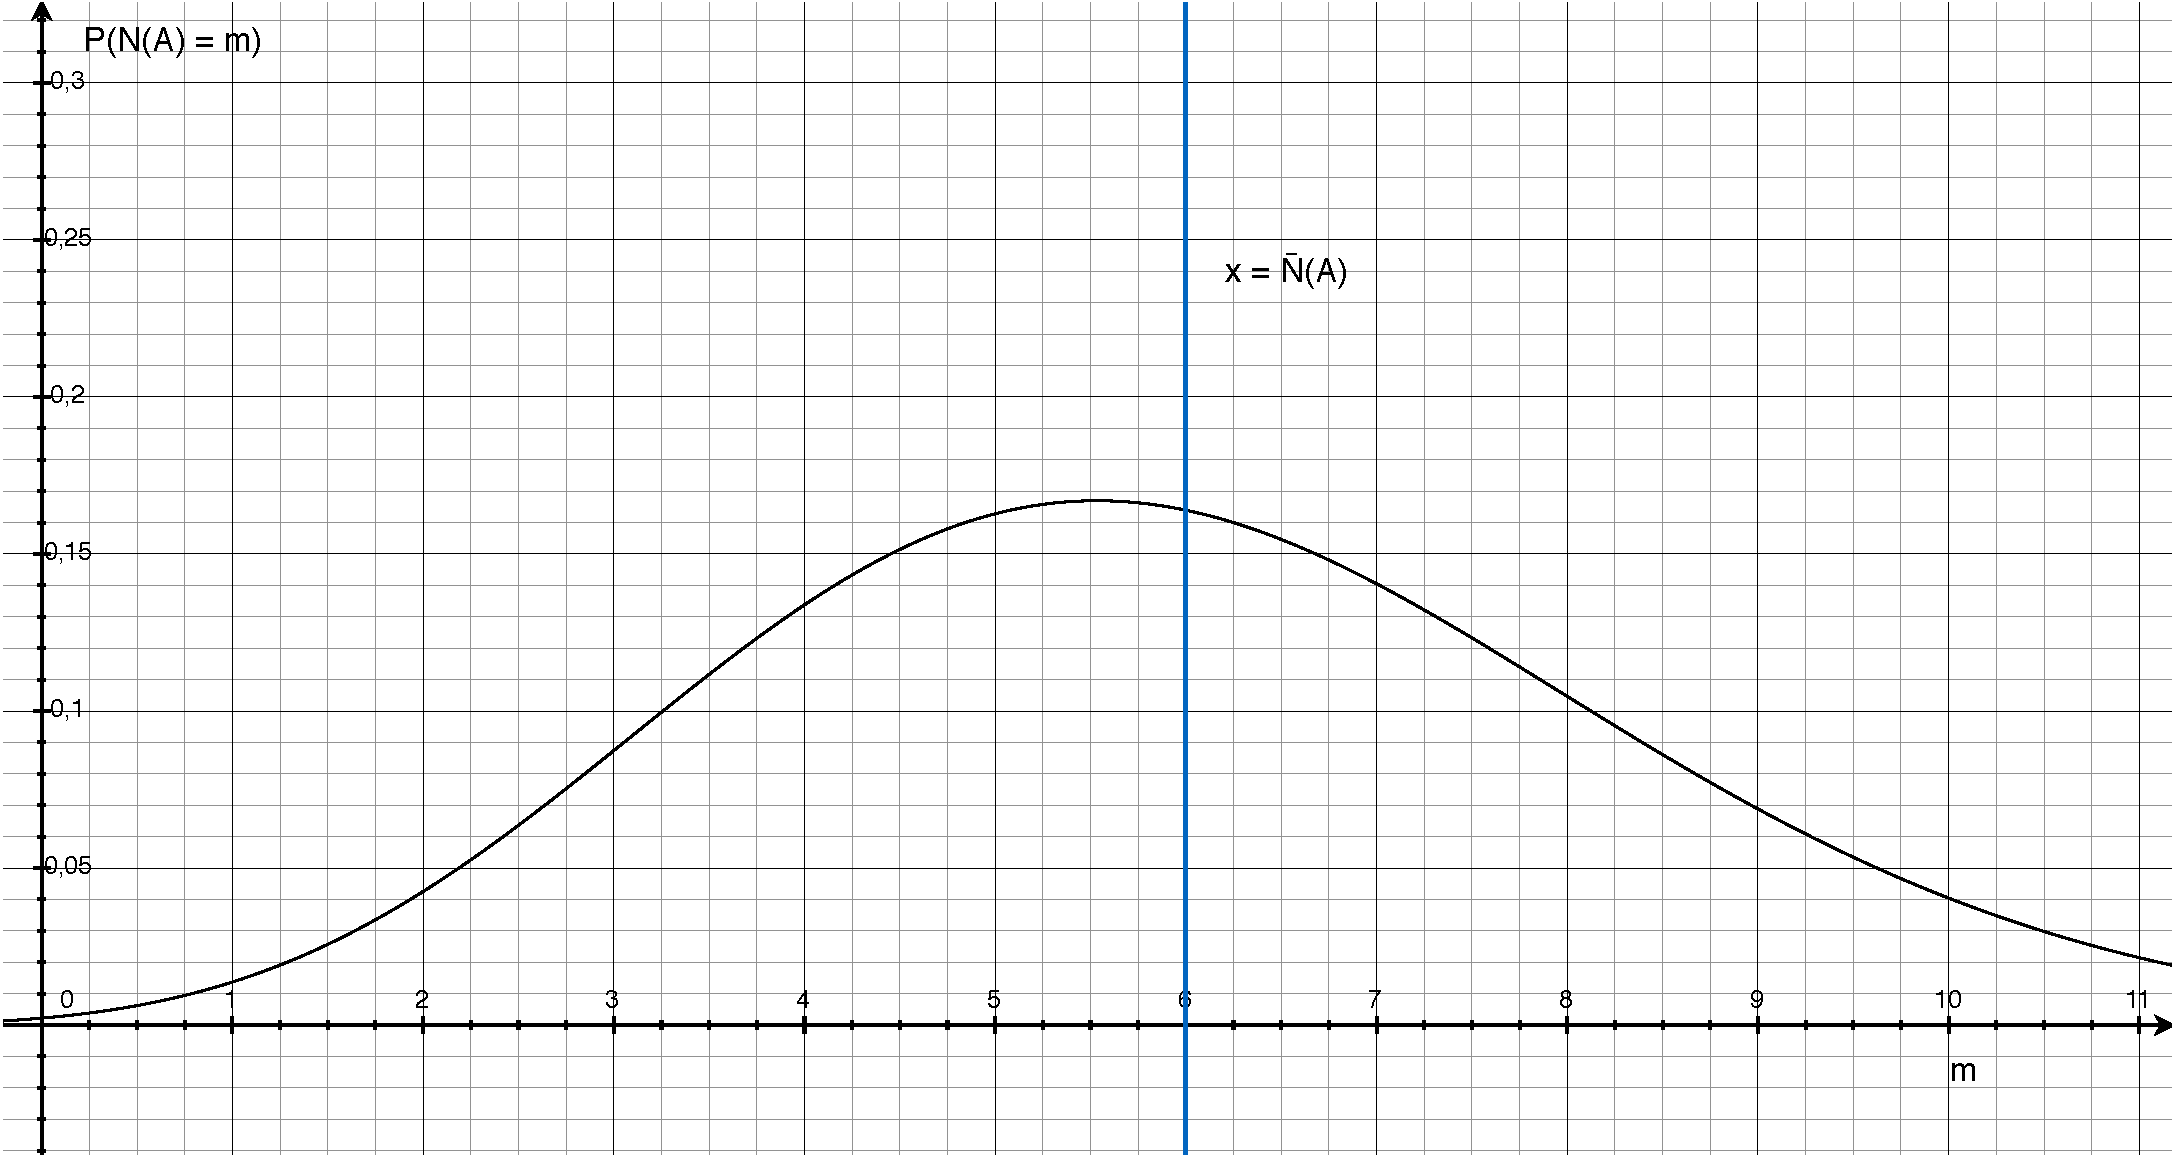
\includegraphics[width=.6\textwidth]{fig/plane_rand_n.pdf}
\caption{$P[N(A) = m]$ for randomly dispersed points on a plane, interpolated to real values}
\label{fig:plane_rand_n}
\end{figure}


\section{Closest point histogram with square grid point dispersion on plane} \label{sec:proof_sqgrid_disp_plane}
Under the assumption of two perfectly aligned planar surfaces $P$ and $Q$, where points on $P$ are arranged on a square grid with surface density $\rho(P)$, the probability density function $f_R$ is
\begin{equation}
f_R(r) = \frac{1}{2 l} \times \begin{cases}
	\frac{\pi}{4} \, r & 0 \leq r \leq \frac{l}{2} \\
	\left( \frac{\pi}{4} - \arctan{\sqrt{\left( \frac{2r}{l} \right)^2 - 1}} \right) r & \frac{l}{2} < r < \frac{l}{2} \sqrt{2}
\end{cases}
\end{equation}
with $l = \frac{1}{\sqrt{\rho(P)}}$.

\begin{proof}
The points are arranged on a square grid, with side length $l$. For the purpose of the following explanation, let $l = 2$.

Figure \ref{fig:sq_grid} shows four points $p_1, p_2, p_3, p_4 \in P$ with two-dimensional coordinates, and a point $q$ that lies on the same plane as those four points. The background color indicates for each position the distance to the closest point of $P$. It remains constant on each of the white contour lines. $d(q, P)$ is maximal when $q$ is in the center of one of the squares, as it does on the figure. So $d_{\text{max}} = \sqrt{2}$.

The histogram corresponds to the probability distribution of $d(q, P)$. The entire plane can be tiled with the triangle $\Delta$ which is drawn in the figure, with the probability distribution being the same in each of these tiles, as the $\Delta$ would only get flipped along one of its sides. So it is sufficient to only look at the field within $\Delta$. Its side lengths are $1, 1, \sqrt{2}$, and its angle at the point $p_1 = (0, 0)$ is $\frac{\pi}{8}$. For each point inside $\Delta$, $p_1$ is its closest point in $P$.

Each value for $d \in [0, d_{\text{max}}]$ occurs in $\Delta$, exactly at the points that lie on the arc formed by the intersection of $\Delta$ and the circle $C_d$ of radius $d$. Let $a(d)$ be the length of this arc in function of $d$. On the figure, $k$ is the intersection point of $\overline{p_1 q}$ with $C_1$. When $d \leq 1$, the arc ranges from the abscissa axis to the diagonal, which is one eight of the circle, and so $a_1(d) = \frac{\pi}{4} \, d$.

When $1 < d < d_{\text{max}}$, it is additionally cut off by the line $x = 1$. By solving $(x, y) \in C_d \wedge x = 1$, its intersection point with that line is $(1, \sqrt{d^2 - 1})$. Instead of starting from the abscissa, the remaining arc now starts from $\varphi = \arctan{\sqrt{d^2 - 1}}$, and so $a_2(d) = (\frac{\pi}{4} - \varphi) \, d$. The function $a$ is
\begin{equation}
a(d) = \begin{cases}
	\frac{\pi}{4} \, d & 0 \leq d \leq 1 \\
	\left( \frac{\pi}{4} - \arctan{\sqrt{d^2 - 1}} \right) \, d & 1 < d < \sqrt{2}
\end{cases}
\end{equation}
under the assumption that $l = 2$.

Removing this assumption, $l$ is now determined as a function of the surface points density $\rho$. The density is constant throughout the surface, so $\rho$ expresses the number of points that lie inside any region of $P$, divided by the area of that region. The area of a square region formed by four points is $l^2$. After a small translation of the point in any direction so that they don't lie on the region's borders, there is $1$ point in each $l^2$ region. So $\rho = \frac{1}{l^2}$ and $l = \frac{1}{\sqrt{\rho}}$. In this general case, the function $a$ becomes
\begin{equation}
a(d) = \frac{l}{2} \times \begin{cases}
	\frac{\pi}{4} \, d & 0 \leq d \leq \frac{l}{2} \\
	\left( \frac{\pi}{4} - \arctan{\sqrt{\left( \frac{2d}{l} \right)^2 - 1}} \right) \, d & \frac{l}{2} < d < \frac{l}{2} \sqrt{2}
\end{cases}
\end{equation}

Since the arcs completely completely cover $\Delta$ and none of them overlap, $\int a(d) \, \diffd d = \area{\Delta} = l^2$. Normalizing the integral to $1$, the probability density function $f_R$ becomes
\begin{equation}
f_R(d) = \frac{a(d)}{l^2}
\end{equation}

\begin{figure}[h]
\centering
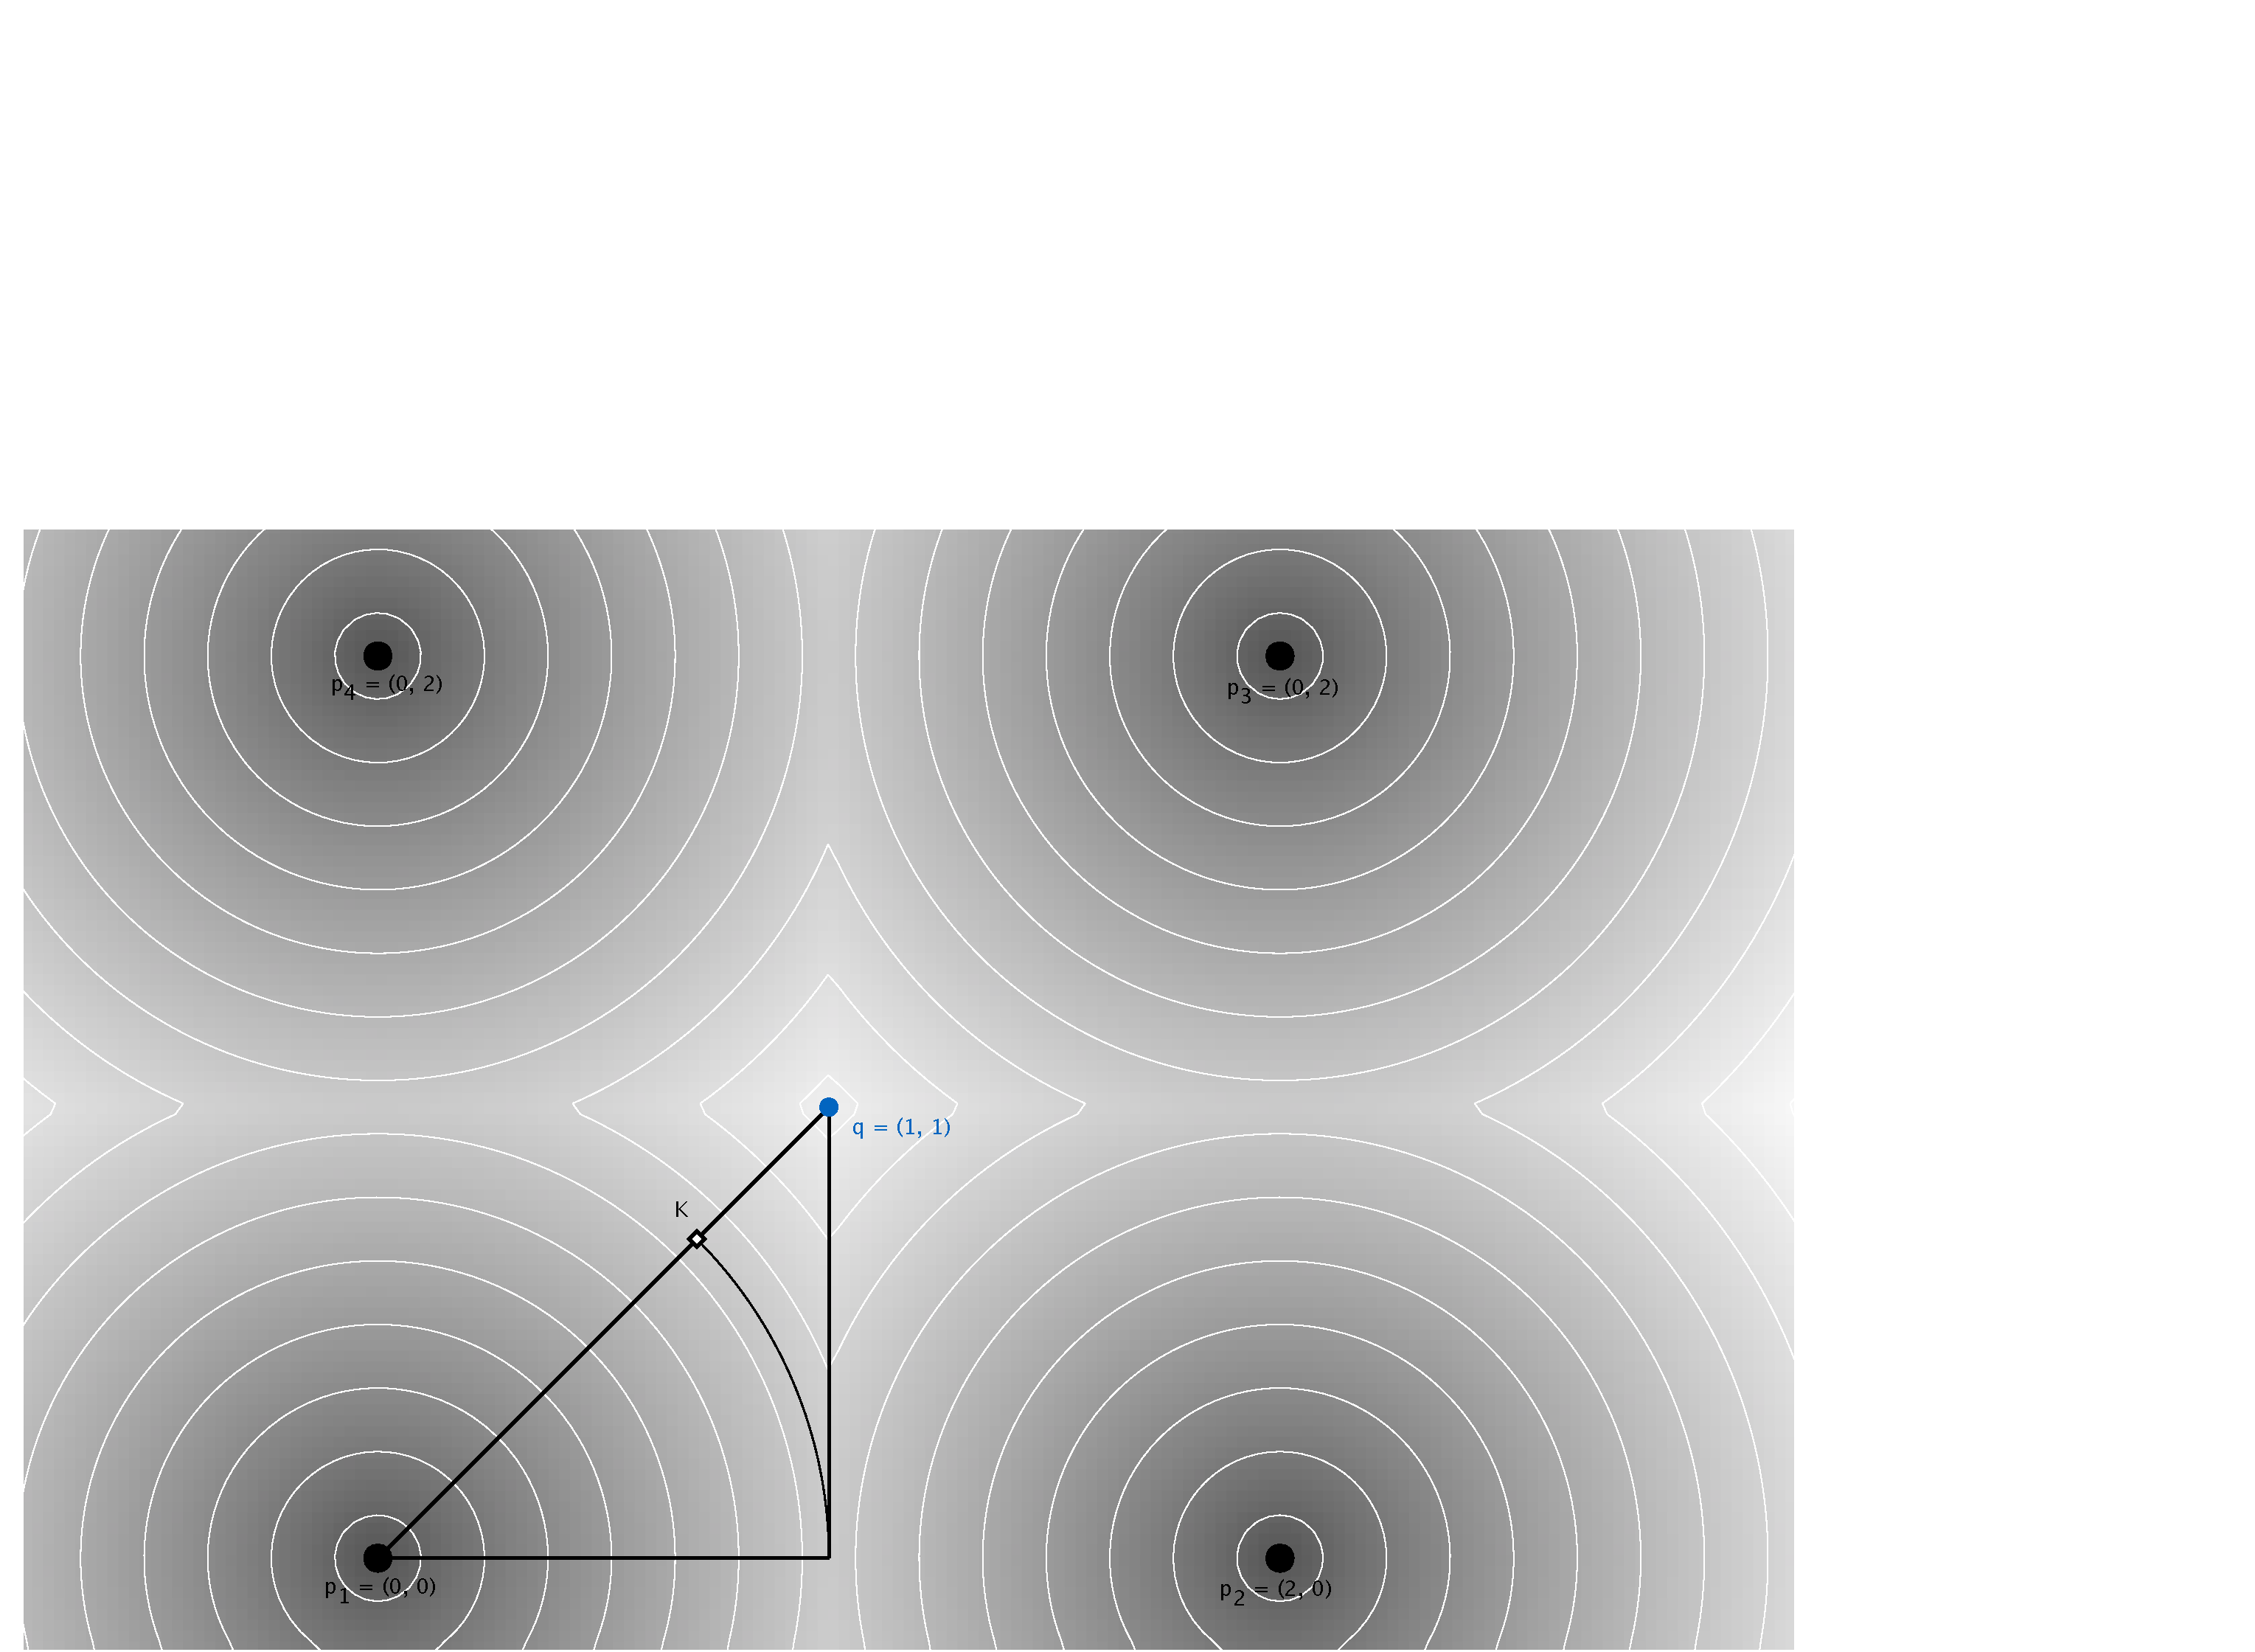
\includegraphics[width=.8\textwidth]{fig/sq_grid.pdf}
\caption{Closest points distance field with square grid distribution of $P$, $l = 2$}
\label{fig:sq_grid}
\end{figure}

\end{proof}
